\documentclass[problem]{mcs}

\begin{pcomments}
  \pcomment{CP_pythagorean}
  \pcomment{ARM 01/30/15 from welcome slides}
\end{pcomments}

\pkeywords{
   proof
   pythagorean
   triangles
   square
   right_angle
   area
}

%%%%%%%%%%%%%%%%%%%%%%%%%%%%%%%%%%%%%%%%%%%%%%%%%%%%%%%%%%%%%%%%%%%%%
% Problem starts here
%%%%%%%%%%%%%%%%%%%%%%%%%%%%%%%%%%%%%%%%%%%%%%%%%%%%%%%%%%%%%%%%%%%%%

\begin{problem}
The Pythagorean Theorem says that if $a$ and $b$ are the lengths of
the sides of a right triangle, and $c$ is the length of its
hypotenuse, then
\[
a^2+b^2 = c^2.
\]
This theorem is so fundamental and familiar that we generally take it
for granted.  But just being familiar doesn't justify calling it
``obvious''---witness the fact that people have felt the need to
devise different proofs of it for milllenia.\footnote{Over a hundred
  different proofs are listed on the mathematics website
  \href{Cut-the-Knot}{http://www.cut-the-knot.org/pythagoras/}.}  In
this problem we'll examine a particularly simple ``proof without
words'' of the theorem.

Here's the strategy.  Suppose you are given four different colored
copies of a right triangle with sides of lengths $a$, $b$ and $c$,
along with a suitably sized square, as shown in Figure~\ref{fig:righttri}.

\begin{figure}[h]
\graphic[height=2.25in]{pythagorean-triangles}
%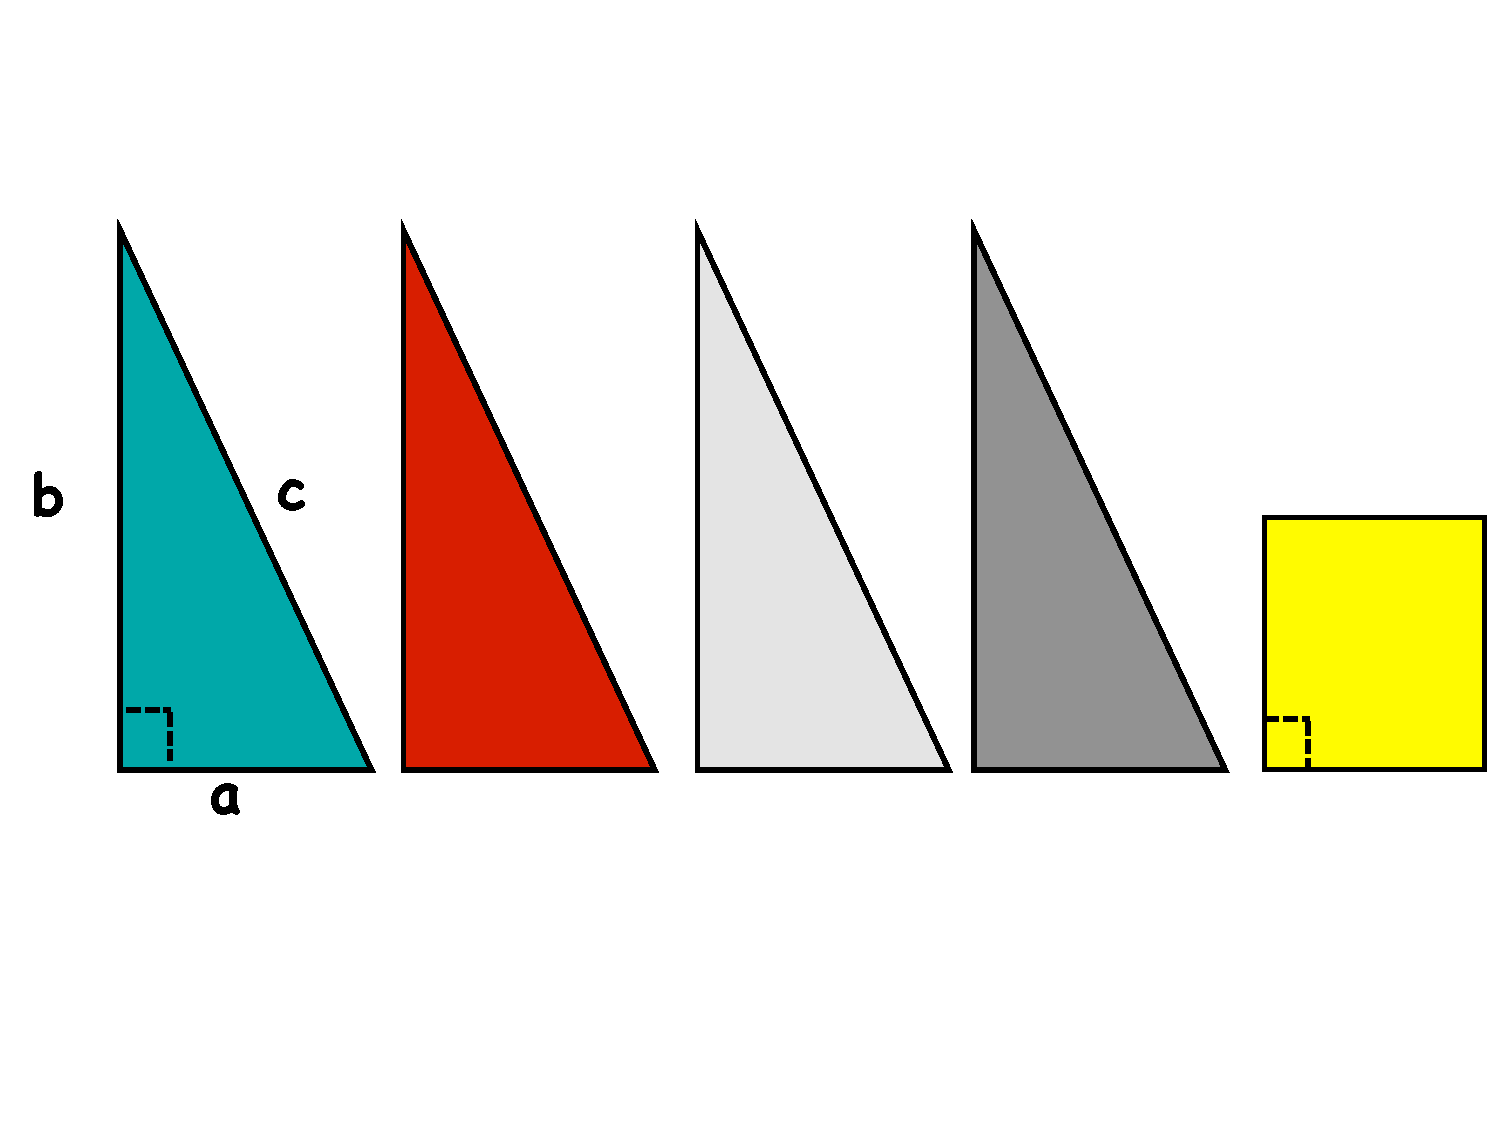
\includegraphics[width=\linewidth]{pythagorean-triangles}
\caption{Right triangles and square.}
\label{fig:righttri}
\end{figure}

\begin{problemparts}
\ppart You will first arrange the square and four triangles so they
form a $c \times c$ square.  From this arrangement you will see that
the square is $(b-a) \times (b-a)$.

\begin{solution}
The arrangement is given in Figure~\ref{fig:cxcsq}.

\begin{figure}[h]
\graphic[height=3in]{cxc-arrangement}
%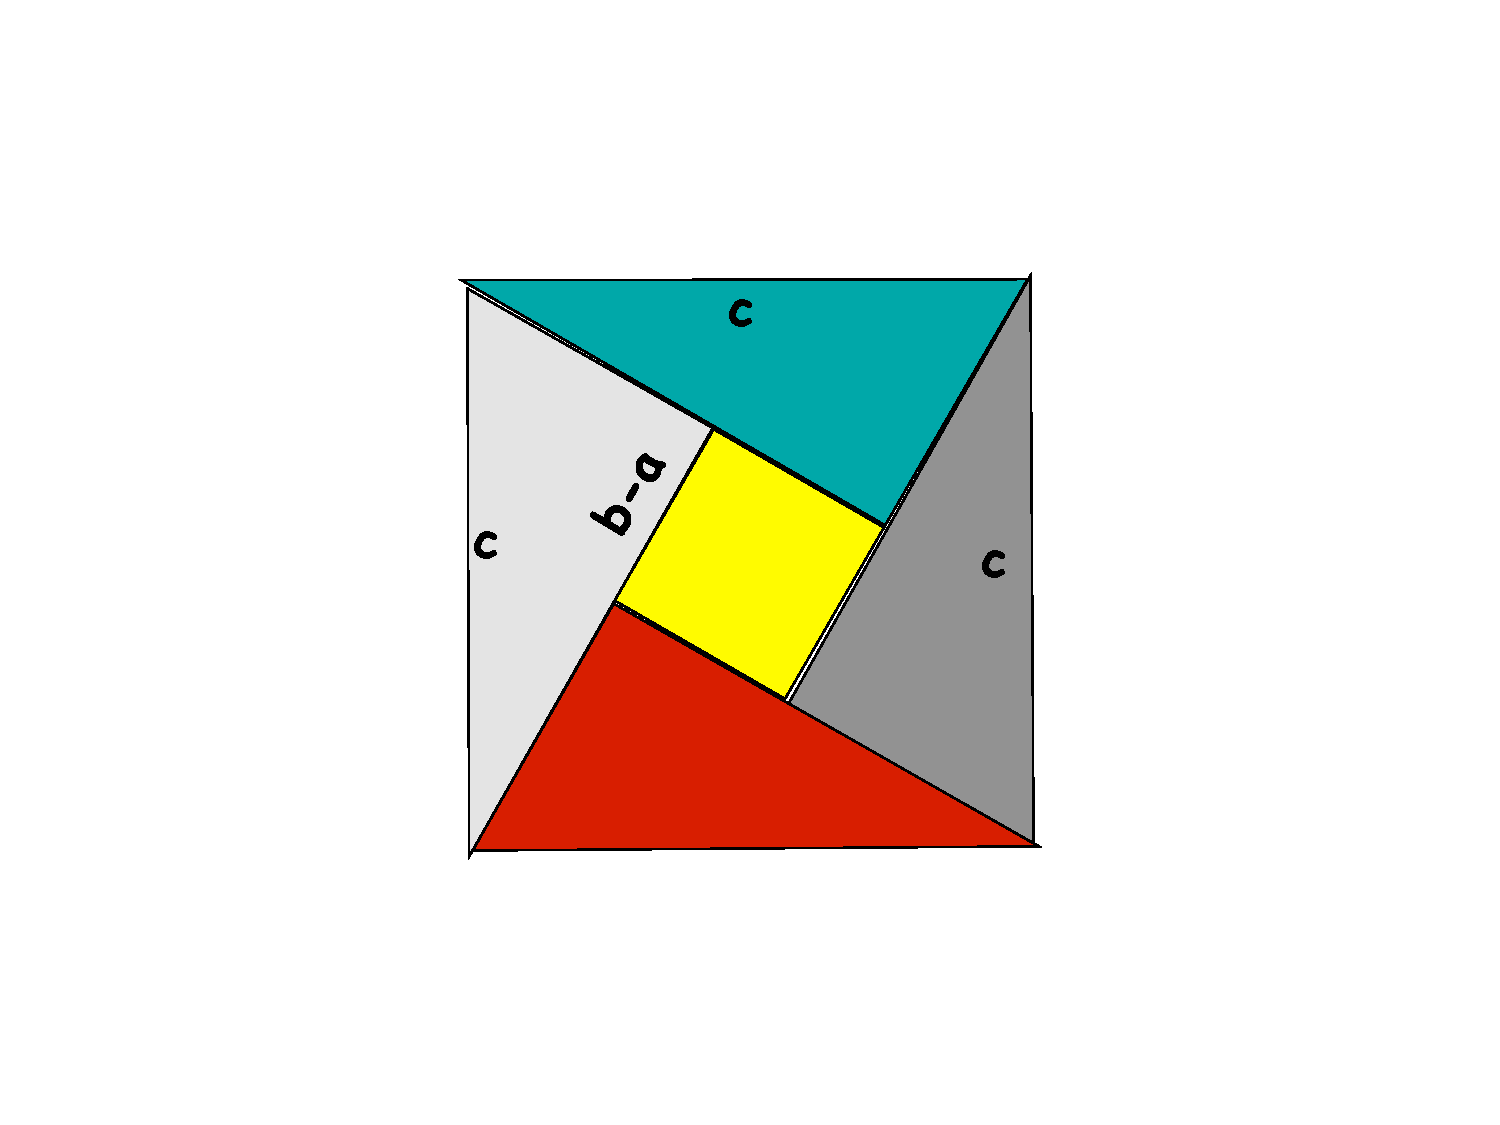
\includegraphics[width=1.2\linewidth]{cxc-arrangement}
\caption{$c \times c$ square.}
\label{fig:cxcsq}
\end{figure}

Notice that the length $a$ side of the red triangle plus the length of
the square side equals the length of the $b$ side of the light gray
triangle, so the square side must be of length $b-a$.

\end{solution}

\ppart You will then arrange the same shapes so they form two squares,
one $a \times a$ and the other $b \times b$.  

\begin{solution}
\hint The two squares are attached.

The arrangement is given in Figure~\ref{fig:axabxb}.

\begin{figure}[h]
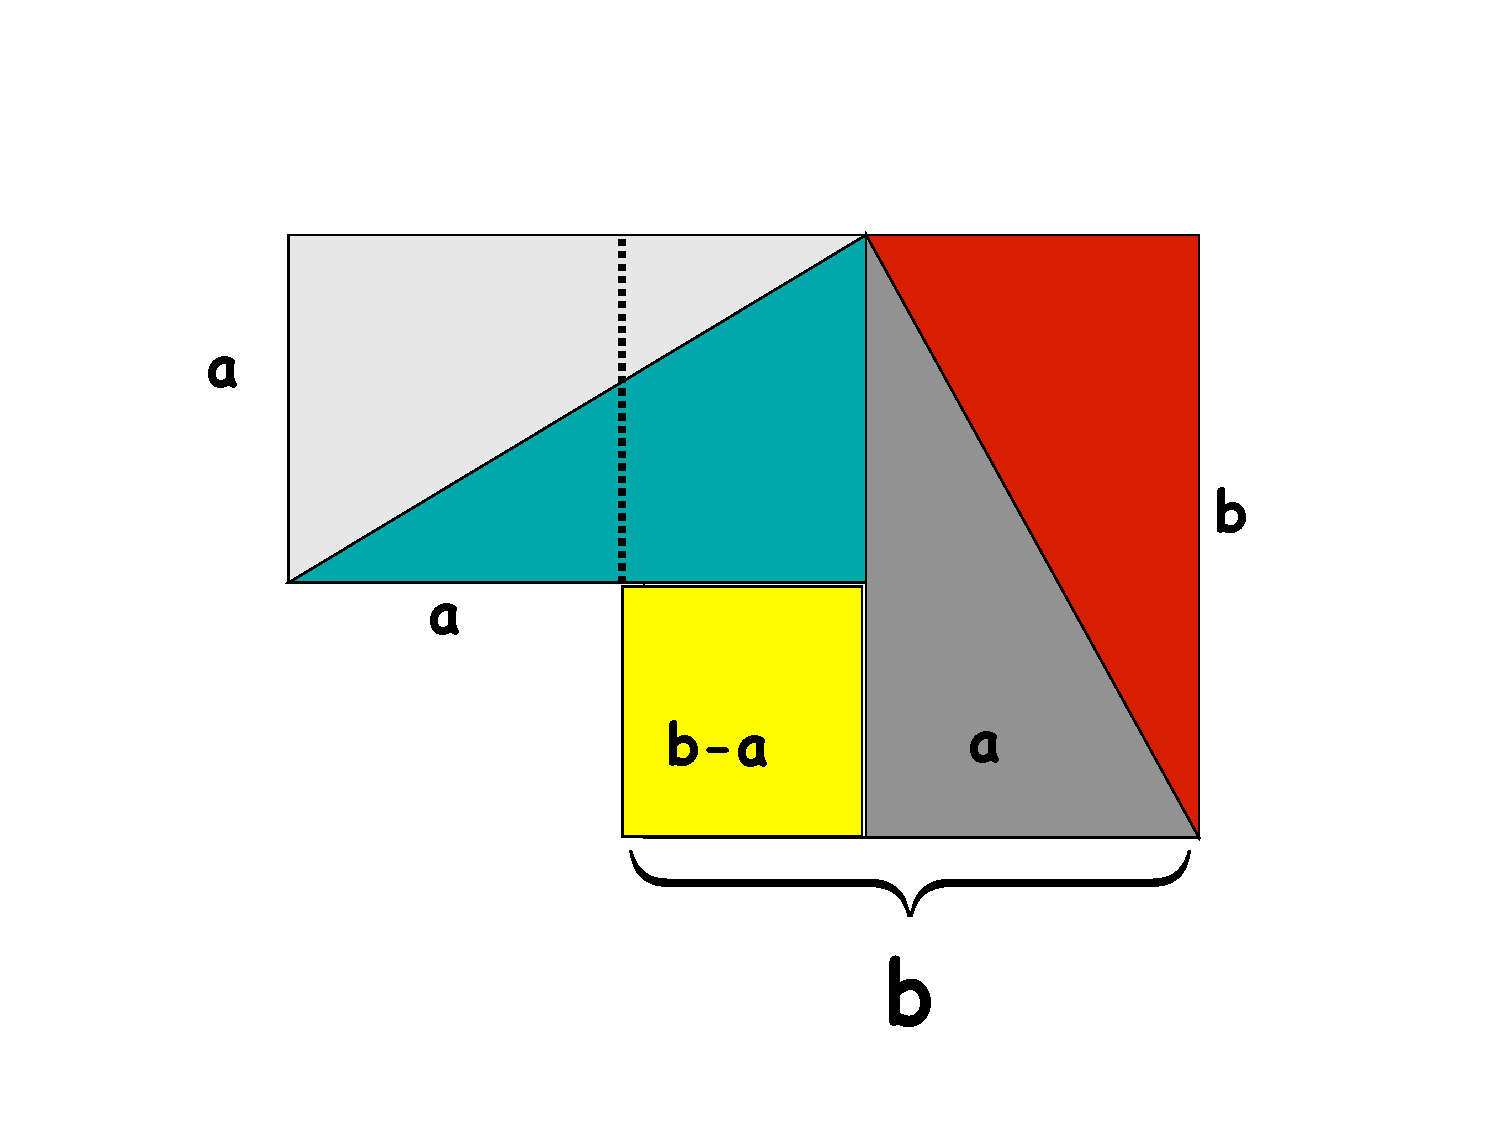
\includegraphics[height=3in]{axa-bxb-arrangement}
%{axa-bxb-arrangement}[width=\linewidth]
\caption{$a \times a$ and $b \times b$ squares.}
\label{fig:axabxb}
\end{figure}
\end{solution}
\end{problemparts}

You know that the area of an $s \times s$ square is $s^2$.  So
appealing to the principle that
\begin{center}
\emph{Area is Preserved by Rearranging},
\end{center}
you can now conclude that $a^2+b^2=c^2$, as claimed.

This really is an elegant and convincing proof of the Pythagorean
Theorem, but it has some worrisome features.  One concern is that
there might be something special about the shape of these particular
triangles and square that makes the rearranging possible---for
example, suppose $a=b$?

\begin{problemparts}

\ppart How would you respond to this concern?

\begin{solution}
The justification for being able to rearrange triangles of arbitrary
shape with a matching square as shown in Figures~\ref{fig:cxcsq}
and~\ref{fig:axabxb} uses only a few basic facts about
triangles, most notably that complementary angles of a right triangle
sum to a right angle.  The case $a=b$ raises no problem in fitting the
shapes together, except that the square reduces to a point with zero
area.

\end{solution}

\ppart Another concern is that a number of facts about right
triangles, squares and lines are being \emph{implicitly} assumed in
justifying the rearrangements into squares.  Enumerate some of these
assumed facts.

\begin{staffnotes}
Don't let students blow this off.  Report to instructors any
additional assumptions students may identify.
\end{staffnotes}

\begin{solution}

\text{}

\begin{itemize}
\item Complementary angles of a right triangle sum to a right angle
  (used in four places in each of Figures~\ref{fig:cxcsq}
  and~\ref{fig:axabxb}).

\item Lining up two right angled corners yields a straight line (also
  used in four places in each of Figures~\ref{fig:cxcsq}
  and~\ref{fig:axabxb}).

\item Lengths along a line add up (used in four places in
  Figure~\ref{fig:cxcsq} and five places in
  Figure~\ref{fig:axabxb}).

\item \dots?

\end{itemize}
\end{solution}

\end{problemparts}

 
\end{problem}

%%%%%%%%%%%%%%%%%%%%%%%%%%%%%%%%%%%%%%%%%%%%%%%%%%%%%%%%%%%%%%%%%%%%%
% Problem ends here
%%%%%%%%%%%%%%%%%%%%%%%%%%%%%%%%%%%%%%%%%%%%%%%%%%%%%%%%%%%%%%%%%%%%%

\endinput
